%% ESANN 2027 submission (STRICT 6 pages, A4, no appendix in proceedings).
%% Regular track, topic: Trustworthy AI. Single blind: names stay.
%% Snapshot 2026-11-13: dagger (†) marks runs still in progress; final numbers in camera-ready.
%% Numbers: paper_numbers.py (deduped, multi-return-guarded) + harvest_examples.json.

\documentclass{esannV2}
\usepackage{graphicx}
\usepackage[utf8]{inputenc}
\usepackage{amsmath,amssymb,array}

\newcommand{\inprog}{$^\dagger$}

\begin{document}

\title{Witness-guided specification\\
repair for trustworthy LLM vericoding}

\author{Patrik P\'ancz\'el, Zolt\'an K\'ar\'asz and L\'aszl\'o Guly\'as
%
\vspace{.3cm}\\
E\"otv\"os Lor\'and University, Faculty of Informatics \\
Budapest, Hungary \\
}

\maketitle

\begin{abstract}
Language models now write both the formal specification and the verified
implementation, and verifier acceptance is routinely reported as success. This
trust is misplaced. Across 2786 instrumented runs on three Dafny benchmarks,
35\% of accepted solutions satisfy a specification that misses the intended
behaviour, and the most capable models are the least reliable. A single solver
query flags these weak specifications far more accurately (F1 0.78) than an LLM
judge (0.41), yet turning any flag into automatic repair breaks more correct
specifications than it fixes. We propose witness-guided repair, which derives a
concrete input on which the specification admits two different outputs, asks
whether the natural-language description permits both, and strengthens the
specification only when it does not, making it the only method that never
damaged a correct specification. The resulting loop outperforms published
pipelines on their own benchmarks, verifying 74\% of MBPP-DFY tasks against the
53--58\% reported for GPT-4, and it reports which of its acceptances deserve
trust.
\end{abstract}

\section{Introduction}

Verification-aware languages such as Dafny give code generation a machine-checkable
acceptance signal, and a growing family of benchmarks scores language models by how
often a verifier accepts their output \cite{dafnybench,verina,vericoding}. In the
increasingly common \emph{vericoding} setting the model generates the specification
too, from a natural-language description, then generates code against its own
specification. The verifier confirms only that the program satisfies the
specification it was handed. If that specification underdetermines the intent,
incorrect programs satisfy it as well, and LLM-written postconditions that
verify yet miss the intent are widely observed \cite{aiassist,specharness}.

Recent work offers individual remedies (completeness filtering, mutation
adequacy, determinacy checks and test-based faithfulness, Sec.~\ref{sec:rw}), but
the works we reviewed deploy such signals for evaluation or data filtering. This
paper asks the trustworthiness question behind them. Can a cheap signal be relied
on to flag an untrustworthy acceptance, and can it be trusted to fix
the specification without damaging correct ones?

The main contributions are the following.
\begin{enumerate}\itemsep1pt\parskip0pt
\item Across 1551 oracle-evaluated acceptances, 35\% do not entail the intended
specification, and reliability is inverted against capability
(Fig.~\ref{fig:dash}a--c).
\item As predictors, a solver determinacy query (F1 0.78) dominates an LLM judge
(0.41) and mutation-style signals (Sec.~\ref{sec:repair}).
\item Every flag-driven repair arm is net-harmful, and we introduce
\emph{witness-guided repair}, the only arm with zero regressions (Sec.~\ref{sec:repair}).
\item Benign non-determinism confounds signals, repair and the evaluation oracle
itself, confirmed by a value-core and an independent test oracle
(Sec.~\ref{sec:repair}).
\end{enumerate}
Against published pipelines on their own benchmarks the resulting loop is
stronger and self-measuring (Fig.~\ref{fig:dash2}). Code and the full
instrumented corpus accompany the paper.

\section{Related work}
\label{sec:rw}

Vericoding benchmarks score acceptance at scale \cite{dafnybench,verina,%
vericoding}. ATLAS filters synthetic data with completeness lemmas \cite{atlas}.
Determinacy checks assess postcondition completeness for deterministic programs
\cite{sast26}. Mutation-based adequacy is studied for Dafny and LLM contracts
\cite{mutdafny,specharness}. Verus-SpecGym measures faithfulness against
test suites \cite{specgym}. Maximal specification inference \cite{maxspec}
supplies the formal backbone our witness arm borrows. Our prior study
\cite{mavcg} found a verified specification can make strong models regress by
underdetermining intent, the inversion this paper measures. Relative to these, we
compare the signals as predictors \emph{and} repair drivers in one loop, add
intent-arbitrated witness repair, and quantify the non-determinism confound at
all three levels.

\section{Methodology}
\label{sec:method}

A task consists of a natural language description $d$ and a hidden reference
postcondition $G$ used only for evaluation. The pipeline produces a candidate
postcondition $S$ and a program $P$ with a verified triple
$\{\mathit{pre}\}\,P\,\{S\}$. Acceptance is a formal statement about $S$ and not
about $G$. An acceptance is reliable when $S \Rightarrow G$ holds.

The determinacy signal asks the solver to prove that $S(x,r_1)$ and $S(x,r_2)$
imply $r_1 = r_2$, and a failed proof flags $S$. The flag alone cannot tell a
weak specification from one that legitimately allows several correct answers, so
the witness step turns it into evidence. By bounded enumeration or by perturbing
$P$'s output on precondition-satisfying inputs we find a concrete triple
$(x, r_1, r_2)$ with $r_1 \neq r_2$ where both pairs satisfy $S$ under execution,
a machine-checked fact with no model opinion. The arbiter receives $d$ and the
witness and decides whether both candidates lie in the intended output set
$O_d(x)$. If so the ambiguity is benign and $S$ is kept. Otherwise the repair
forms $S' = S \wedge C$ rejecting the witnessed wrong output, so $S'$ implies $S$
and can only shrink the admitted behaviours. The implementation is reverified
against $S'$ and on failure the previous state is kept. Without a witness, a
behavioural branch generates proof-free implementations from $d$ and sends any
disagreement with $P$ to the same arbiter and a guarded rewrite.

Three properties make the design trustworthy. Every flag reaching the arbiter is
backed by an executable or verified fact, so the evidence is sound. Breaking a
correct specification would need both an arbiter error and a verified
overconstrained specification, which keep-on-fail precludes. And the pipeline
never sees $G$, so the method is answer-key-free.

\section{The pipeline}
\label{sec:setup}

Figure~\ref{fig:pipe} shows the full loop. From the method signature and the
natural-language description the model generates a postcondition. A syntax
gate validates it with the verifier's parser and feeds concrete parse errors back
(at most twice). Without it, 48\% of all failures began with an
unparseable specification poisoning every later step. The model then generates an
implementation with up to five verifier-feedback iterations. A task is
accepted when the implementation verifies, mirroring standard practice
\cite{vericoding,atlas}.

On every acceptance the trust layer computes five answer-key-free signals
(determinacy \cite{sast26,atlas}, output perturbation \cite{atlas}, program
mutation \cite{mutdafny}, mined invariants, LLM judge \cite{specgym}) and runs
the repair arms. Evaluation uses three held-out oracles (Sec.~\ref{sec:method}),
namely entailment against the curated postcondition, a non-determinism-aware
value-core oracle and the benchmark's executable tests where available.

\textbf{Corpus and models.} Three Dafny families from the vericoding corpus
\cite{vericoding}, \texttt{numpy\_simple} (58), \texttt{verina} (157) and
\texttt{verified\_cogen} (172 tasks), each with a curated held-out specification.
The snapshot covers nine models, claude-opus-5-5, gpt-6-astra, claude-sonnet-4-6,
grok-4.3 and qwen2.5-coder~32B complete and claude-opus-4-6, gpt-5, gpt-5-mini,
gpt-oss~20B in progress\inprog, with two more queued\inprog.

\begin{figure}[t]
\centering
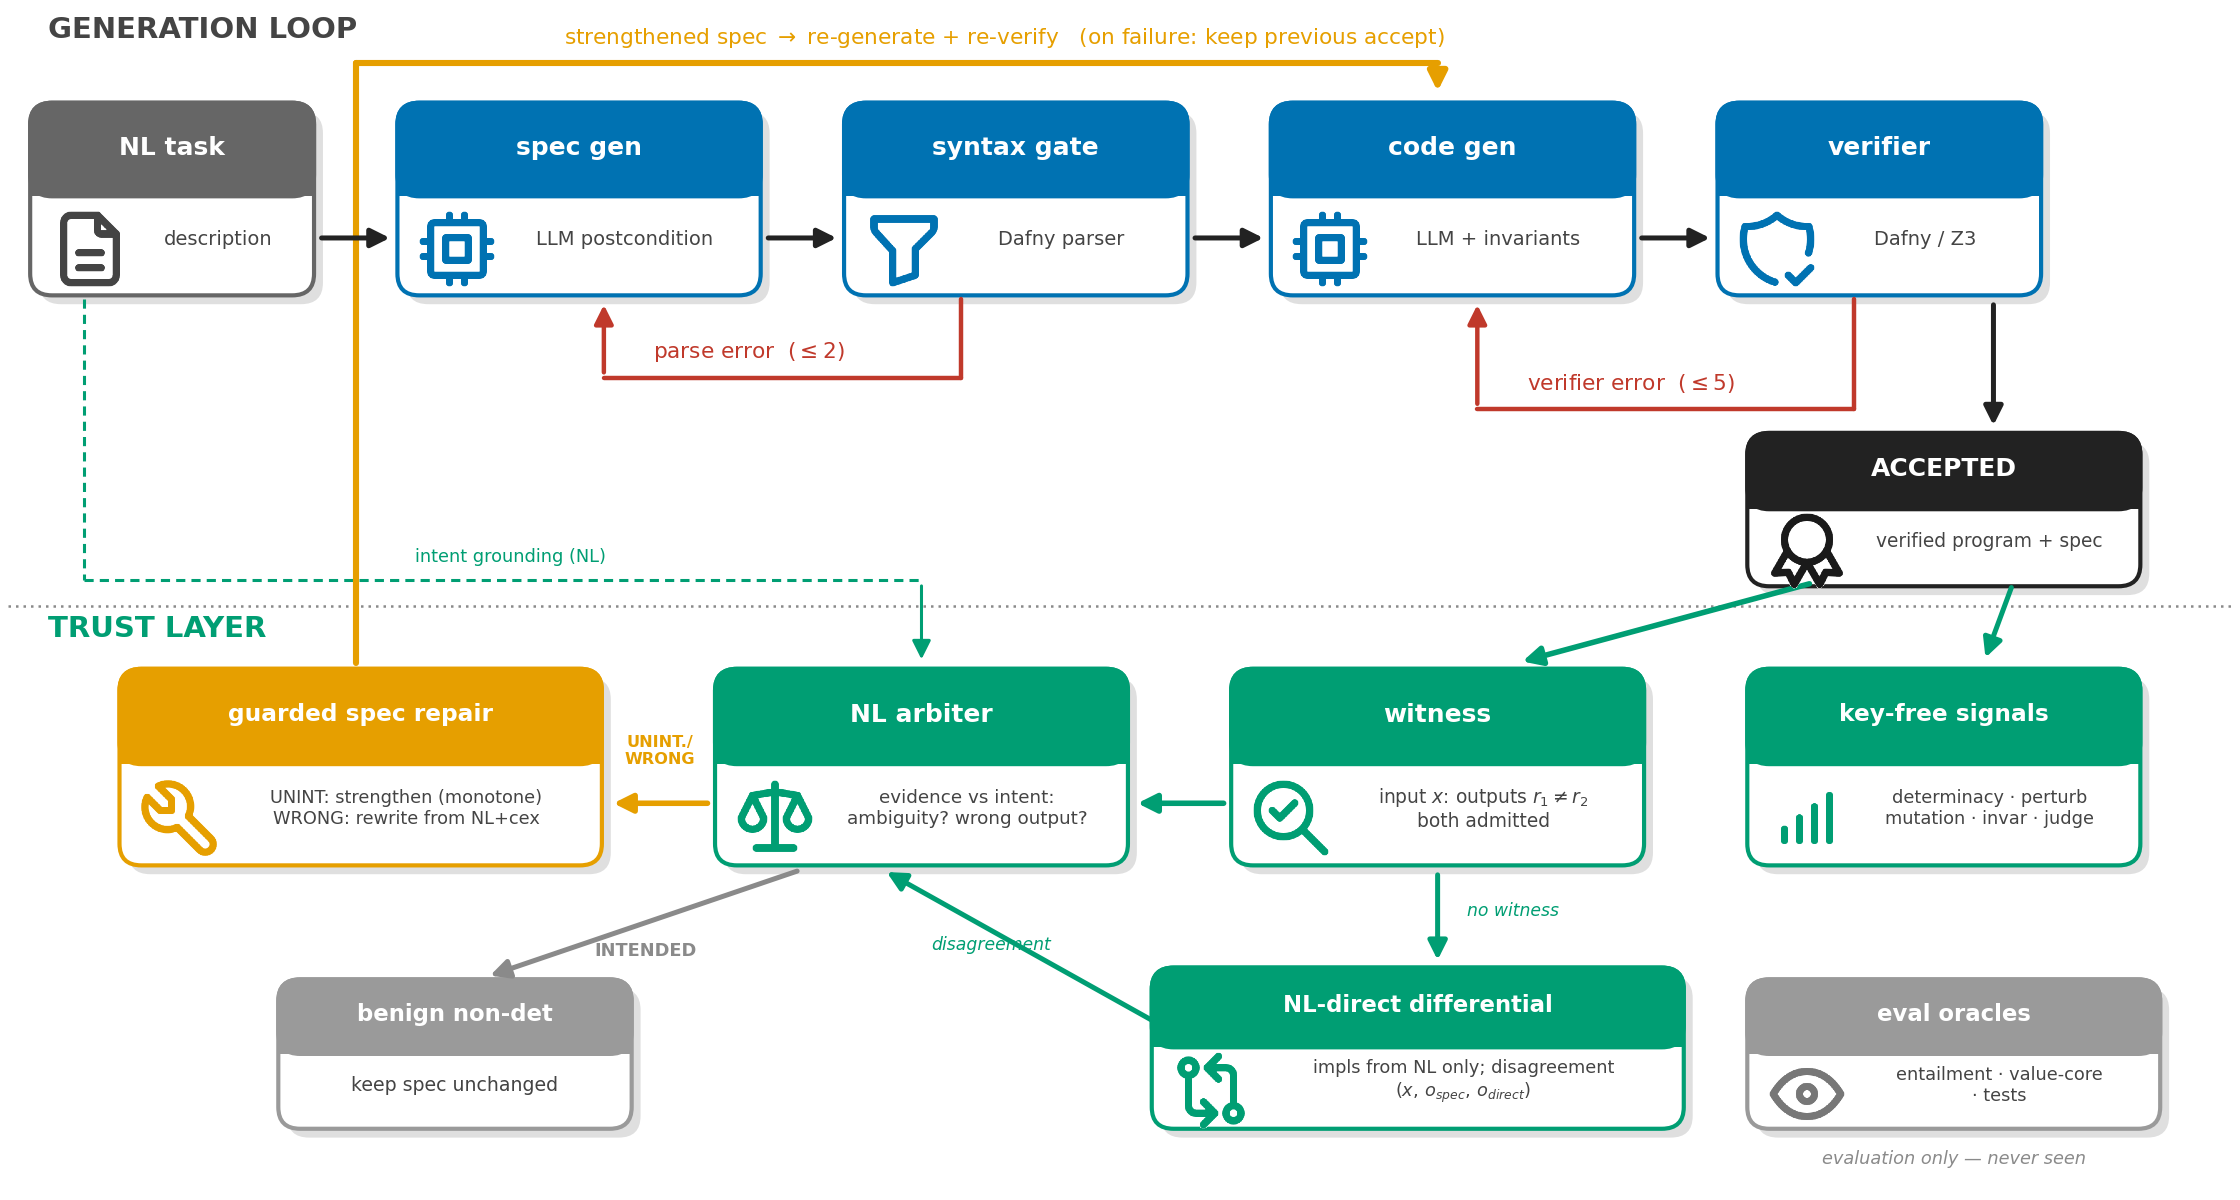
\includegraphics[width=\textwidth]{fig22_pipeline.png}
\caption{The instrumented vericoding loop. Red marks standard error feedback. The
trust layer (ours) poses formally grounded questions (an ambiguity \emph{witness},
or a behavioural disagreement with implementations generated from the NL alone)
and lets the NL description arbitrate intent (dashed). Benign ambiguity is kept,
unintended ambiguity is strengthened monotonically, wrong specifications are
rewritten from the NL plus the counterexample, and on any re-verification failure
the previous accepted state is kept.}
\label{fig:pipe}
\end{figure}

\section{Acceptance is not correctness}
\label{sec:accept}

Of 1551 evaluated acceptances, 1002 (65\%) entail the intended specification,
while 35\% verify against a specification permitting unintended behaviour (55\%,
70\% and 63\% reliable by benchmark). Reliability inverts against capability
(Fig.~\ref{fig:dash}a), with claude-opus-5-5 accepting 98\% of tasks at 65\%
reliability while qwen2.5-coder accepts 29\% at 72\%. A stronger generator is
better at finding some verifying pair, including one whose specification is
conveniently weak, so scoring acceptance alone flatters the strongest models
most, up to 39 points of overstated verified-rate for gpt-6-astra
(Fig.~\ref{fig:dash}b,c). The vericoding benchmark these families come from
\cite{vericoding} reports 30--83\% acceptance across nine LLMs with no
reliability measure, and its own manual inspection flags weak or mistranslated
specifications among accepts, on the same tasks we score.

The external oracles concur. On MBPP-DFY \cite{aiassist}, six verified acceptances
fail the dataset's own tests (e.g.\ task~264). Conversely,
thirteen entailment-``unreliable'' acceptances pass all tests, so the oracle,
not the code, is sometimes wrong
(Sec.~\ref{sec:repair}). Three further acceptances entail the curated specification
yet fail tests, so even curated specifications are occasionally incomplete.

\section{Flagging works, flag-driven repair harms}
\label{sec:repair}

As predictors of unreliable acceptance the signals differ sharply.
Determinacy reaches F1 0.78 (precision 0.76, recall 0.81),
the LLM judge, despite seeing the task, misses two thirds of the weak
specifications (F1 0.41), mutation suffers from equivalent mutants and
perturbation almost never fires. A single solver query with no tests and no extra
LLM call is the best flag.

Turning flags into repair fails. With five rounds of
strengthening and code re-verification, the invariant arm repairs 12 of its 505
intervention targets while breaking 60, the determinacy arm 27 against 53 of 589,
and the judge 17 against 121 of 421, so 29\% of its interventions destroy a
correct specification. The dominant cause is benign non-determinism. Among
flagged-weak acceptances, 50\% have an intended specification that admits several
correct outputs, 43\% of determinacy's false alarms and 45\% of its repair
breakage sit on this class, and a flag-driven loop strengthens such
specifications past the intent.

Witness-guided repair (Sec.~\ref{sec:method}) feeds back evidence instead of a
flag. On the snapshot it activated 57 times, stopped at 23 benign verdicts,
repaired 3 and broke none, the only zero-regression arm.

{\footnotesize\textbf{Caught.} ``Find the index of the maximum element.''
Generated \texttt{0\,$\le$\,result\,$<$\,|arr|} $\wedge$ \texttt{arr[i]\,$\le$\,arr[result]}
admits on witness \texttt{arr=[0,0,0,-2]} both \texttt{result=0} \emph{and}
\texttt{2}. The arbiter rules UNINTENDED (``the index'' is singular) and adds
\texttt{arr[j]=arr[result]${\Rightarrow}$j$\ge$result}, the reference's
first-maximum convention.\par
\textbf{Spared.} NpArgsort admits \texttt{[0,1]} and \texttt{[1,0]} on
\texttt{a=[3,3]}, the arbiter rules INTENDED and leaves it, correctly.\par}

\textbf{The confound reaches the oracle.} Entailment demands the benchmark's
arbitrary tie-breaking, so a correct any-maximum repair fails a first-maximum
reference. A \emph{value-core} oracle (correct observable values
$a[\mathit{result}]$, after \cite{maxspec}) vindicates 14 of 57 index-returning
``unreliable'' verdicts (72\%$\to$91\%) and re-ranks the arms. The invariant arm
swings from $-12$ to $+2$, the witness arm stays net-positive under \emph{both}
oracles, and the MBPP test oracle agrees (Sec.~\ref{sec:accept}).

\begin{figure}[t]
\centering
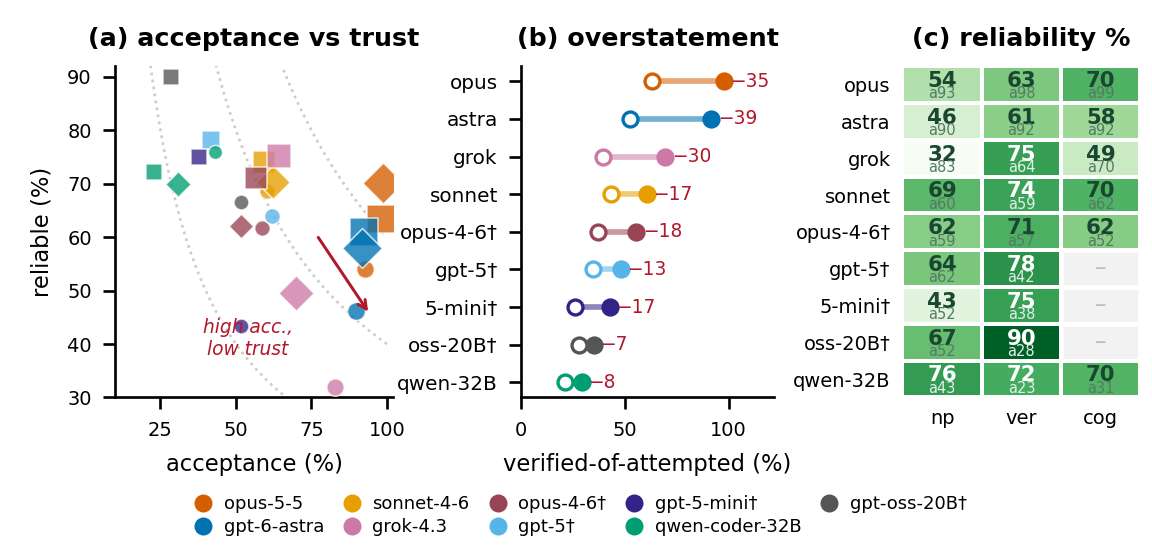
\includegraphics[width=\textwidth]{fig23a_results.png}
\caption{Corpus snapshot ($\dagger$ = run in progress). (a) higher acceptance,
lower reliability (dotted = equal reliable throughput). (b) raw vs
reliability-corrected verified rate. (c) reliability per model and benchmark
(large) with acceptance (small, \texttt{a}).}
\label{fig:dash}
\end{figure}

\begin{figure}[t]
\centering
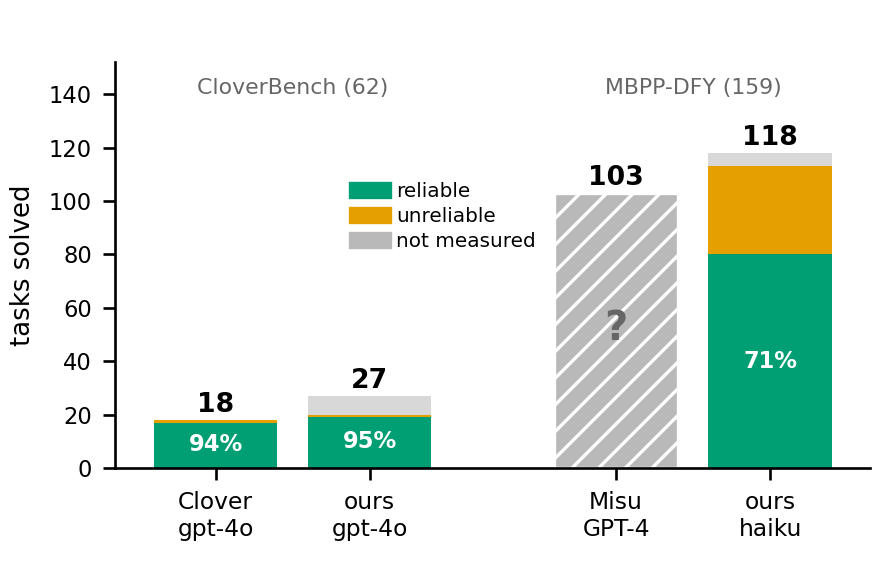
\includegraphics[width=.78\textwidth]{fig23b_results.png}
\caption{Accepts per pipeline, each at its own acceptance gate, on CloverBench
(vs Clover, both gpt-4o) and MBPP-DFY (vs \cite{aiassist}, ours claude-haiku-4-5).
Green reliable, orange unreliable, hatched not measured.}
\label{fig:dash2}
\end{figure}

\section{Against published pipelines}
\label{sec:external}

\textbf{Clover} \cite{clover} accepts when code, docstring and annotation are
mutually consistent. On its own 62-task CloverBench with both pipelines on gpt-4o,
Clover's consistency gate accepts 18 specifications at \textbf{94\%} reliability,
while our loop accepts 27 at \textbf{95\%} (19 of the 20 with a reference), and
the NL-differential branch concurs. At matching precision our deductive proof
admits 50\% more tasks, resolving cases a consistency score leaves open. Clover's
raw specifications, before its gate, are only 56\% reliable, so the gate itself
does real work, the same lesson our trust layer applies.

On \textbf{MBPP-DFY} the authors \cite{aiassist} report 53--58\% verified
synthesis with GPT-4. Our loop with the budget claude-haiku-4-5 verifies
\textbf{74\%} (118 of 159 applicable tasks) and quantifies its own
trustworthiness. Of the 113 accepts with a reference, 71\% entail the curated
specification, and of all 118, 51 pass and 6 fail the tests (61 inconclusive).

\section{Conclusions}

Acceptance by a verifier is routinely read as correctness, yet a third of
acceptances do not entail the intent and the gap grows with capability. For
flagging, one solver query beats an LLM judge at negligible cost and we recommend
reporting determinacy-filtered alongside raw acceptance. For fixing, repair must
first do no harm, and separating under-specification from benign non-determinism
achieves this with zero regressions. Extending witness extraction and value-core
oracles beyond integer-like returns is the direct next step, which our
instrumented corpus supports.

% ,- references ,-
\begin{thebibliography}{9}
\scriptsize\setlength{\itemsep}{-3.4pt}

\bibitem{dafnybench} C.~Loughridge, et~al. DafnyBench: A Benchmark for Formal
Software Verification. \emph{arXiv:2406.08467}, 2024.

\bibitem{verina} Z.~Ye, et~al. VERINA: Benchmarking Verifiable Code Generation.
\emph{arXiv:2505.23135}, 2025.

\bibitem{vericoding} S.~Bursuc, et~al. A Benchmark for Vericoding: Formally
Verified Program Synthesis. \emph{arXiv:2509.22908}, 2025.

\bibitem{atlas} M.~Baksys, S.~Zetzsche, et~al. ATLAS: Automated Toolkit for
Large-Scale Verified Code Synthesis. \emph{arXiv:2512.10173}, 2025.

\bibitem{sast26} C.~V.~P.~Silveira, M.~Tymburib\'a. Postcondition Completeness in
Auto-Generated Function Contracts. \emph{Proc. SAST}, 2026.

\bibitem{mutdafny} MutDafny: A Mutation-Based Approach to Assess Dafny
Specifications. \emph{arXiv:2511.15403}, 2025.

\bibitem{specharness} Spec-Harness: Behavioral Adequacy of LLM-Synthesized Formal
Specifications. \emph{arXiv:2604.00280}, 2026.

\bibitem{specgym} Verus-SpecGym: Evaluating Specification Autoformalization.
\emph{arXiv:2605.26457}, 2026.

\bibitem{clover} C.~Sun, Y.~Sheng, et~al. Clover: Closed-Loop
Verifiable Code Generation. \emph{Proc. SAIV}, 2024.

\bibitem{maxspec} A.~Albarghouthi, I.~Dillig, A.~Gurfinkel. Maximal Specification
Synthesis. \emph{Proc. POPL}, 2016.

\bibitem{aiassist} M.~Misu, et~al. Towards AI-Assisted Synthesis of Verified
Dafny Methods. \emph{Proc. FSE}, 2024.

\bibitem{mavcg} P.~P\'ancz\'el, L.~Guly\'as. MAVCG: Model-Assisted Verified Code
Generation from ODD Protocols via Dafny Specifications.
\emph{Proc. Intelligent Robotics FAIR}, ACM, 2026.

\end{thebibliography}

\end{document}
